% - O que é Modelagem Matemática de um problema (características);
% - O que é um problema de otimização e pra que ela serve;
% - O que é otimização discreta e otimização contínua;
% - Os tipos de programação de cada uma delas;


\section{Otimização}

% escrever aqui uma introdução a otimização, passando pela apresentação dos termos centrais e sobre modelagem matemática

% É uma área da Pesquisa Operacional1 com vasta aplicação em apoio à decisão, pois muitos problemas reais podem ser modelados como problemas de PL.

%1 Pesquisa Operacional é o conjunto de conhecimentos relacionados com o processo científico de tomada de decisão, aplicados no projeto e operação de sistemas homem-máquina, em um ambiente com recursos restritos.

% Um vetor x∗ ∈ S é dito ser uma solução ótima ou ponto de ótimo do problema de minimizar f se satisfaz a condição f (x∗ ) ≤ f (x) para todo x ∈ S . (2)

% REVER APRESENTAÇÃO DO CLAUDIO/RAFA. BEM INTERESSANTE A ORDEM! <<<<<<

% PROBLEMA DOS FRANGOS NA GRANJA. 
% suponha que queremos fazer algumas alterações no processo de engorda dos frangos para que possamos aumentar nossa produtividade. Mas é muito caro ficar fazendo os testes, ou até mesmo inviável, em tempo de produção. Para contornar esse problema, recorremos a modelagem matemática, onde aproximamos o problema real para um problema matemático, onde podemos controlar e testar nossas variáveis livremente e estimar os resultados.
% essa modelagem pode ser complexa. Nesse exemplo, estamos interessados em estudar a interação entre cada frango na granja, o que se assemelha muito aos problemas moleculares, regidos pelas diversas forças entre átomos da molécula.


% Apresentar a introdução a modelagem modelando um problema real. Aos moldes do que Martinez fez, devemos apresentar um problema que eu tenha domínio. Bom, deve ser o problema de geometria de distâncias moleculares.. ou o problema de carteiras ótimas. Vamos ver.


A \textit{modelagem} é a área de estudo que objetiva descrever fenômenos do mundo real por meio de ferramentas matemáticas, servindo de conexão entre a matemática e as outras áreas do conhecimento \cite{meerschaert2013mathematical}. Partindo de problemas encontrados na física, engenharia, química, biologia e outras ciências, busca-se caracterizar e compreender seus comportamentos através de variáveis, funções e outras ferramentas matemáticas, abstraindo a situação real com o cuidado de que não se percam os comportamentos de interesse. Quanto mais variáveis e restrições são incorporadas para descrever os comportamentos do sistema real, mais fidedigna, porém complexa, torna-se sua representação. Grande parte da pesquisa realizada nessa área pode ser dividida em três categorias: modelos probabilísticos, modelos dinâmicos e modelos de otimização. Nos concentraremos no terceiro.

A otimização é uma área da pesquisa operacional que da suporte na tomada de decisões, com o objetivo de encontrar soluções \textit{ótimas} para um problema. Uma \textit{solução ótima} (ou \textit{ponto ótimo}) é aquela que \textit{minimiza} ou \textit{maximiza} uma função $f$, chamada de \textit{função objetivo} do problema (Figura~\ref{fig:otimizacao}). Simbolicamente, dizemos que $x^* \in \mathcal{X}$ é \textit{solução ótima} do problema de minimizar $f$, restrito a $\mathcal{X}$, se satisfaz $$f(x^*)\leq f(x)\text{ para todo } x\in \mathcal{X}.$$ O conjunto $\mathcal{X}$ é chamado de \textit{espaço de busca} por uma solução, e encontrar essa solução ótima nem sempre é fácil ou mesmo possível. Isso gera a necessidade do estudo de \textit{aproximações} para as soluções ótimas de um problema \cite{elizabeth2013otimizaccao}.  

Perceba que o problema de maximizar $f$ é equivalente ao de minimizar $-f$ (veja Figura~\ref{fig:max_min_equiv}), o que nos permite abster de comentários sobre um dos dois nas definições e proposições que seguem. Com lealdade à abordagem defendida pelos colegas da Unicamp, focaremos exclusivamente nos problemas de minimização, deixando os equivalentes de maximização como exercício para o leitor. 

\begin{figure}[h]
    \centering
    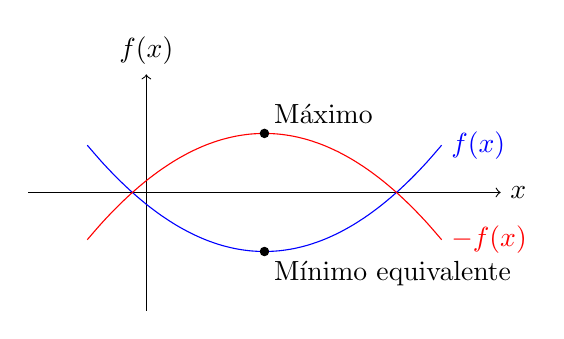
\begin{tikzpicture}[scale=1.5]
        % Eixo x
        \draw[->] (-1,0) -- (3,0) node[right] {$x$};
        % Eixo y
        \draw[->] (0,-1) -- (0,1) node[above] {$f(x)$};
        % Função f(x)
        \draw[domain=-0.5:2.5,smooth,variable=\x,blue] plot ({\x},{0.4*(\x-1)^2 - 0.5}) node[right] {$f(x)$};
        % Função -f(x)
        \draw[domain=-0.5:2.5,smooth,variable=\x,red] plot ({\x},{-0.4*(\x-1)^2 + 0.5}) node[right] {$-f(x)$};
        % Ponto máximo
        \filldraw[black] (1,0.5) circle (1pt) node[above right] {Máximo};
        % Ponto mínimo equivalente
        \filldraw[black] (1,-0.5) circle (1pt) node[below right] {Mínimo equivalente};
    \end{tikzpicture}
    \caption{Maximizar $f(x)$ é equivalente a minimizar $-f(x)$.}
    \label{fig:max_min_equiv}
\end{figure}

\begin{figure}[h]
	\centering
	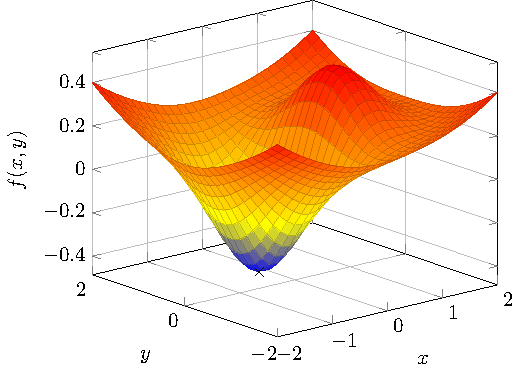
\includegraphics[scale=0.9]{secOtimizacao/figures/solucaoOtima.pdf}
	\caption{Ilustração do problema de minimização para a função objetivo $f:\mathbb{R}^2\to\mathbb{R}$, definida pelo mapeamento $(x,y) \mapsto xe^{-x^2-y^2} + \frac{x^2 + y^2}{20}$.}
	\label{fig:otimizacao}
\end{figure}
	
Um problema geral de otimização é representado como 
\begin{mini}
	{x\in \mathcal{X}}{f(x)}{}{}
\end{mini}
onde $x$ é o vetor de variáveis contidas no \textit{espaço de busca} $\mathcal{X} \subset \mathbb{R}^n$, candidatas a solução. Dependendo da natureza do problema, podemos representar o conjunto $\mathcal{X}$ através de restrições de igualdade e de desigualdade, ou seja,
$$\mathcal{X} = \{x\in \mathbb{R}^n\ |\ c_\mathcal{E}(x) = 0,\ c_\mathcal{I}(x) \leq 0\},$$
onde $c_\mathcal{E}: \mathbb{R}^n\to\mathbb{R}^m$ e $c_\mathcal{I}: \mathbb{R}^n\to\mathbb{R}^p$ são as \textit{funções de restrição} do espaço de busca $\mathcal{X}$ e $0$ representa os vetores nulos de dimensão apropriada\footnote{A menos de ambiguidades, omitiremos as dimensões de vetores nulos e identidades.}.
Para destacar as restrições do problema, iremos escrevê-lo como 
\begin{mini}
	{x\in \mathbb{R}^n}{f(x)}{}{}
	\addConstraint{c_\mathcal{E}(x) = 0}
	\addConstraint{c_\mathcal{I}(x) \leq 0.}
\end{mini}

No entanto, caso $\mathcal{X} = \mathbb{R}^n$, dizemos que esse é um \textit{problema de otimização irrestrito}. Também, o conjunto de pontos de $\mathcal{X}$ que satisfazem todas as funções de restrição são chamados de \textit{conjunto factível} (ou viável) do problema.

Em princípio, podemos intercambiar restrições de igualdade e desigualdade livremente, já que restrições de igualdade podem ser reescritas como duas de desigualdade
$$h(x)=0 \quad \iff \quad \begin{matrix}
	\ h(x) \leq 0\\
	-h(x)\leq 0,
\end{matrix}$$
e restrições de desigualdade podem ser reescritas como de igualdade, mediante a introdução de variáveis artificiais ``de folga''
$$g(x) \leq 0 \quad \iff \quad g(x) + z^2 = 0,\ z\in \mathbb{R}. $$
Infelizmente, as transformações desse tipo não são desejadas nem do ponto de vista teórico nem do ponto de vista computacional \cite{izmailov2005otimizaccao}.

\begin{exemplo}[Lei de Hooke]
	Considere um problema de engenharia mecânica em que estamos projetando uma mola para que ela exiba um comportamento elástico ideal de acordo com a Lei de Hooke. A tarefa é determinar a espessura da mola, representada por $x$, de modo a minimizar a energia potencial elástica armazenada na mola.

	A Lei de Hooke estabelece que a energia potencial elástica, $U$, é diretamente proporcional ao quadrado do deslocamento da mola, ou seja, $U(x) = \frac{1}{2}kx^2$, onde $k$ é a constante da mola. Nosso objetivo é minimizar a energia potencial $U$ sujeita a um limite na espessura da mola, ou seja, $a \leq x \leq b$, onde $a$ e $b$ são valores específicos que respeitam as características do projeto.
	
	Portanto, nosso problema de otimização é modelado como:
	\begin{mini}
		{x\in \mathbb{R}}{\frac{1}{2}kx^2}{}{}
		\addConstraint{x\geq a}
		\addConstraint{x\leq b}
	\end{mini}
	Neste exemplo, o espaço de busca é o intervalo $[a, b]$, a função objetivo é a energia potencial elástica, e não há restrições adicionais além dos limites da espessura da mola. Este é um exemplo de um problema de otimização contínua em $\mathbb{R}$.
\end{exemplo}


No exemplo acima, restringimos o espaço de busca $\mathbb{R}$ no intervalo factível $[a,b]$, cuja continuidade induz uma busca contínua por valores ótimos nesse intervalo. Problemas desse tipo são chamados de \textit{problemas de otimização contínua}. Em contraste, quando nosso espaço de busca é um subconjunto dos inteiros $\mathbb{Z}$, ou, mais geralmente, quando o conjunto de restrições é tal que nosso espaço factível é um conjunto enumerável de pontos, diremos que esse é um \textit{problema de otimização discreta}.

\textbf{Exemplo (Problema da Mochila).} Suponha que estamos enfrentando o "Problema da Mochila", um desafio clássico na otimização combinatória. Nesse cenário, temos um conjunto de itens com pesos $w_i$ e valores $v_i$, juntamente com uma mochila que suporta um peso máximo $W$. O objetivo é determinar quais itens devem ser colocados na mochila de forma a maximizar o valor total dos itens, respeitando a restrição de peso.

O problema pode ser formulado da seguinte maneira:
$$\max_{x_i \in \{0, 1\}} \sum_{i=1}^{n} v_i \cdot x_i$$
sujeito a
$$\sum_{i=1}^{n} w_i \cdot x_i \leq W$$
onde $x_i$ é uma variável binária que indica se o item $i$ é selecionado ou não.

Neste exemplo, o espaço de busca consiste em um conjunto finito de pontos (0 ou 1) para cada item, tornando-o um problema de otimização discreta, ou seja, um problema de programação inteira. O objetivo é selecionar os itens de forma a maximizar o valor total, respeitando a restrição de peso máximo da mochila.

Além dos problemas de otimização contínua e discreta, existe uma categoria intermediária conhecida como programação mista. Esses problemas incorporam tanto variáveis contínuas quanto discretas em suas formulações, criando um desafio único. Enquanto os exemplos anteriores lidavam exclusivamente com variáveis contínuas ou discretas, problemas de programação mista requerem a combinação de técnicas de otimização contínua e programação inteira para encontrar soluções que satisfaçam todas as restrições e objetivos do problema.

No contexto da otimização, além das distinções entre otimização contínua, discreta e programação mista, é fundamental compreender as abordagens de otimização global e local. Problemas de otimização muitas vezes requerem a identificação da melhor solução possível, mas essa 'melhor solução' pode variar dependendo da abordagem utilizada. A otimização global se concentra na busca pela solução globalmente ótima, ou seja, aquela que otimiza a função objetivo em todo o espaço de busca, considerando todas as possíveis combinações de variáveis. Por outro lado, a otimização local visa encontrar soluções ótimas dentro de uma região restrita do espaço de busca, muitas vezes iniciando a busca a partir de um ponto inicial. A distinção entre otimização global e local é crucial, uma vez que problemas de otimização podem ter múltiplos ótimos locais, e a escolha entre abordagens global e local depende dos objetivos do problema e das características da função objetivo.

\subsection{Preliminares}
%  write preliminars section to mathematical analisys needed to optimization                              1.1
%2024-02-25 calculus, linear algebra, topology?

% Aqui vamos introduzir a álgebra linear aplicada (avançada)